\documentclass[11pt]{article}
\usepackage[a4paper,margin=25mm]{geometry}
\usepackage{amsmath,booktabs,graphicx,hyperref}
\usepackage[numbers,sort&compress]{natbib}
\usepackage{microtype}
\setlength{\emergencystretch}{2em}
\hypersetup{colorlinks=true,urlcolor=blue,citecolor=blue,linkcolor=blue}
% Generated; edit scripts/data, not this file.
\newcommand{\IssueCount}{1371}
\newcommand{\BugLabelCount}{773}
\newcommand{\BugClosedCount}{756}
\newcommand{\BugOpenCount}{17}
\newcommand{\BugNotPlannedCount}{71}
\newcommand{\BugDuplicateCount}{2}
\newcommand{\BugClosureMedian}{14.76}
\newcommand{\PRCount}{2166}
\newcommand{\HumanPRCount}{1667}
\newcommand{\HumanPRMerged}{1318}
\newcommand{\HumanPRUnmergedClosed}{287}
\newcommand{\HumanPROpen}{62}
\newcommand{\PilotPRCount}{76}
\newcommand{\PilotHumanPRCount}{59}
\newcommand{\PilotResponseCount}{51}
\newcommand{\PilotMergeNoResponse}{3}
\newcommand{\PilotCloseNoResponse}{4}
\newcommand{\PilotNoResponseOpen}{1}
\newcommand{\EvidenceIssueCount}{100}
\newcommand{\EvidenceBotClosures}{29}
\newcommand{\EvidenceClosingCommits}{5}
\newcommand{\EvidenceReopened}{2}
\newcommand{\EvidencePostClosureDiscussion}{19}
\newcommand{\EvidenceCommitRefEvents}{254}
\newcommand{\EvidenceCommitRefCases}{26}
\newcommand{\EvidenceDistinctCommitRefs}{243}
\newcommand{\EvidenceLocalCommitRefs}{48}
\newcommand{\EvidenceMergeCommitLinkedCases}{10}
\newcommand{\EvidenceMergeCommitLinkedPRs}{12}
\newcommand{\ClosingCommitKeywordCases}{5}
\newcommand{\ClosingCommitKeywordMatches}{2}
\newcommand{\RepairValidatedCases}{2}
\newcommand{\RepairRegressionChecks}{3}
\newcommand{\RepairControlChecks}{2}
\newcommand{\RepairGoVersion}{1.24.0}
\newcommand{\MergerAccountCount}{5}
\newcommand{\RoleQuarterPRs}{87}
\newcommand{\RoleQuarterAuthors}{14}
\newcommand{\RoleQuarterMergers}{2}
\newcommand{\RoleQuarterAuthorHHI}{0.545}
\newcommand{\RoleQuarterMergerHHI}{0.700}
\newcommand{\SelfMergeCount}{783}
\newcommand{\ReviewRecordCount}{3073}
\newcommand{\ReviewAccountCount}{54}
\newcommand{\MergedReviewedCount}{1259}
\newcommand{\MergedReviewCoverage}{95.52}
\newcommand{\UnknownReviewActorRecords}{212}
\newcommand{\UnknownReviewActorHumanPRs}{84}
\newcommand{\MissingIdentityFixedPRs}{1259}
\newcommand{\MissingIdentityAffectedPRs}{74}
\newcommand{\MissingIdentityRetainedRecords}{177}
\newcommand{\MissingIdentityAffectedQuarters}{4}
\newcommand{\MissingIdentityQTwoLower}{0.079}
\newcommand{\MissingIdentityQTwoUpper}{0.599}
\newcommand{\MissingIdentityQTwoAuthor}{0.333}
\newcommand{\MissingIdentityQTwoIntegrator}{0.732}
\newcommand{\MissingIdentityQTwoDistinctScenario}{0.079}
\newcommand{\ReviewQuarterAccounts}{4}
\newcommand{\ReviewQuarterPairs}{97}
\newcommand{\ReviewQuarterFractionHHI}{0.388}
\newcommand{\ReviewQuarterPairHHI}{0.386}
\newcommand{\JuanQuarterAuthoredPRs}{0}
\newcommand{\JuanQuarterReviewedPRs}{50}
\newcommand{\GoQuarterPRs}{63}
\newcommand{\GoQuarterAuthorHHI}{0.710}
\newcommand{\GoQuarterReviewerHHI}{0.470}
\newcommand{\GoQuarterIntegratorHHI}{0.939}
\newcommand{\FirstFormalReviewCount}{1323}
\newcommand{\FirstFormalMergeNoReview}{57}
\newcommand{\FirstFormalCloseNoReview}{237}
\newcommand{\FirstFormalOpenNoReview}{50}
\newcommand{\ReopenedHumanPRs}{42}
\newcommand{\FirstClosedEventuallyMerged}{31}
\newcommand{\InitialEpisodeMergeCount}{1287}
\newcommand{\InitialEpisodeClosedCount}{319}
\newcommand{\InitialEpisodeOpenCount}{61}
\newcommand{\ClockDisagreementPRs}{160}
\newcommand{\ClockMaxDelta}{2}
\newcommand{\CoxEarlyCensors}{3}
\newcommand{\CloseReopenTransitions}{45}
\newcommand{\ShortCloseReopenTransitions}{32}
\newcommand{\CoalescedModifiedPRs}{30}
\newcommand{\CoalescedMergeCount}{1313}
\newcommand{\CoalescedConstantHR}{0.997}
\newcommand{\CoalescedConstantLower}{0.926}
\newcommand{\CoalescedConstantUpper}{1.073}
\newcommand{\CoalescedLateHR}{1.308}
\newcommand{\CoalescedLateLower}{1.116}
\newcommand{\CoalescedLateUpper}{1.534}
\newcommand{\CoalescedLateMerges}{66}
\newcommand{\InfluenceQuarterCount}{23}
\newcommand{\InfluenceConstantMin}{0.974}
\newcommand{\InfluenceConstantMax}{1.013}
\newcommand{\InfluenceLateMin}{1.226}
\newcommand{\InfluenceLateMax}{1.373}
\newcommand{\CoxObservationCount}{1661}
\newcommand{\CoxMergeEventCount}{1284}
\newcommand{\CoxQuarterClusters}{23}
\newcommand{\CoxConcentrationHR}{0.998}
\newcommand{\CoxConcentrationLower}{0.927}
\newcommand{\CoxConcentrationUpper}{1.074}
\newcommand{\PieceEarlyHR}{0.984}
\newcommand{\PieceEarlyLower}{0.912}
\newcommand{\PieceEarlyUpper}{1.062}
\newcommand{\PieceLateHR}{1.270}
\newcommand{\PieceLateLower}{1.057}
\newcommand{\PieceLateUpper}{1.527}
\newcommand{\PieceLateMergeEvents}{56}
\newcommand{\PieceNoBacklogLateHR}{1.269}
\newcommand{\PieceNoBacklogLateLower}{1.059}
\newcommand{\PieceNoBacklogLateUpper}{1.521}
\newcommand{\StratifiedConcentrationHR}{0.996}
\newcommand{\StratifiedConcentrationLower}{0.927}
\newcommand{\StratifiedConcentrationUpper}{1.071}
\newcommand{\PilotReopenedPRs}{7}
\newcommand{\PilotDraftHistoryPRs}{12}
\newcommand{\ValidatedCoreAliases}{4}
\newcommand{\QuarterRawHHI}{0.536}
\newcommand{\QuarterLinkedHHI}{0.920}
\newcommand{\QuarterAuthorClockHHI}{0.920}
\newcommand{\OldTopAuthor}{48.16}
\newcommand{\NewTopAuthor}{54.78}
\newcommand{\OldCommitCount}{2803}
\newcommand{\NewCommitCount}{3401}
\newcommand{\OldAuthorCount}{238}
\newcommand{\NewAuthorCount}{259}

\title{Contribution Concentration and Maintenance Outcomes:\\A Longitudinal Case Study of Headscale}
\author{Xiaoyu SHEN\\
\small University of Nottingham Ningbo China\\
\small Provisional contact: \href{mailto:George.Zhou@nottingham.edu.cn}{George.Zhou@nottingham.edu.cn}\\
\small Corresponding author to be confirmed}
\date{Working draft, 14 October 2026}
\begin{document}
\maketitle
\begin{abstract}
Repository activity, maintenance responsibility and repair
outcomes describe different phenomena. We investigate these distinctions in
Headscale, a self-hosted implementation of the Tailscale control server.
Our reproducible case study combines release-pinned Git history,
\IssueCount{} issues, a separate census of \PRCount{} pull requests (PRs),
a complete submitted-review and lifecycle census, a comment-process sample of
\PilotPRCount{} PRs, and evidence for \EvidenceIssueCount{} issues.
We examine author identity, file renaming,
closure mechanisms and competing PR outcomes before interpreting maintenance
trends. Linking validated core-contributor aliases changes production-code author
concentration in 2026 Q2 from Herfindahl--Hirschman index (HHI)
\QuarterRawHHI{} to \QuarterLinkedHHI{}.
The issue evidence sample contains \EvidenceBotClosures{} automated final
closures and only \EvidenceClosingCommits{} explicit closing-commit links,
with component checks supporting \RepairValidatedCases{} local repair links.
Closure alone cannot establish repair.
On the same \RoleQuarterPRs{} merged PRs in 2026 Q2, author, reviewer and
integrator HHIs are \RoleQuarterAuthorHHI{}, \ReviewQuarterFractionHHI{}
and \RoleQuarterMergerHHI{}; review credit is shared per PR.
Observed other-account submitted reviews occur on \MergedReviewedCount{}
of \HumanPRMerged{} human-authored merged PRs. Reopening matters:
\FirstClosedEventuallyMerged{} PRs initially close but subsequently merge.
An exploratory cause-specific model of initial processing episodes estimates a merge hazard ratio
of \CoxConcentrationHR{} per 0.1 increase in prior integration HHI
(95\% interval \CoxConcentrationLower{}--\CoxConcentrationUpper{}).
Elapsed-time diagnostics suggest heterogeneous associations.
These measurements support concentrated activity and heterogeneous closure
mechanisms, without establishing a causal scaling crisis. Independent defect
adjudication and explanatory mechanism validation remain pending. The case
motivates separating activity, responsibility
and outcome boundaries when evaluating vendor-adjacent open-source maintenance.
\end{abstract}
\noindent\textbf{Keywords:} Empirical software engineering; open-source maintenance;
contribution roles; pull requests; issue closure; mining software repositories.

\section{Introduction}
Open-source infrastructure can attract many contributors while remaining dependent
on a small maintenance core. Yet contributor growth alone does not establish
that review, integration and defect handling have become more distributed.
Conversely, concentrated contributions can reflect specialised expertise rather
than declining capacity. An empirical account needs to distinguish these competing
interpretations and establish what its measurements actually observe.

Headscale provides a useful context for this problem. It implements an open-source,
self-hosted Tailscale control server. Its stated scope centres on self-hosters,
hobbyists and smaller organisations, rather than unrestricted parity with the
commercial service~\cite{headscale_design}. A maintainer's FOSDEM presentation
describes the project's growth, upstream funding and protocol relationship
with Tailscale~\cite{dalby2026fosdem}. We use that account as contextual evidence;
we do not treat it as independent verification of repository-derived conclusions.
The upstream client, deployment configuration and server implementation also
create distinct responsibility boundaries for reports filed in one issue tracker.

The motivating pilot observed growth in nominal contributors, a late increase
in commit concentration and longer issue-closure durations. Such a pattern raises
a maintenance question, but cannot answer it by itself. File modifications need
not correspond to coordination handoffs; a closed bug-labeled issue need not
represent repaired server code; and multiple author emails need not identify
different people. We therefore audit the measurements before developing an
explanation of the project's trajectory.

We provide matched comparisons of author, reviewer and integrator activity under
different artifact scopes; time-ordered models of initial PR processing episodes;
and traceable issue evidence separating closure from supported repair.
Release-pinned reproduction and identity/path audits support these measurements.
The results describe this case; the proposed explanation connecting maintenance
roles with client, server and deployment boundaries still requires independent
semantic validation.

\section{Related work and analytical framing}
Headscale has already been evaluated as a research subject.
Kjorveziroski et al. compare it with Netbird and ZeroTier in a full-mesh VPN
performance study, measuring throughput and Kubernetes API response under
adverse network conditions~\cite{kjorveziroski2024mesh}. Their question concerns
deployed-system performance, whereas ours concerns longitudinal repository
maintenance. Selecting Headscale therefore does not itself supply novelty.

Code ownership has long been examined in relation to software quality.
Bird et al. studied ownership and failures in industrial systems, showing that
ownership is an empirical construct requiring specific operationalisation
and validation~\cite{bird2011ownership}. Their results do not justify interpreting
every concentration statistic as knowledge loss or maintenance debt.
Research on coordination breakdowns similarly concerns coordination requirements
and observed process failures, rather than the elapsed time between unrelated
edits by different authors~\cite{cataldo2013coordination}.

Jabrayilzade et al. combine reviews, meetings and version-control activity for
bus-factor estimation and validate against engineer assessments on 13
projects~\cite{jabrayilzade2022bus}. Their discussion already identifies senior
reviewers who contribute little authored code. Our observed author/reviewer
discrepancies illustrate that established concern; they do not introduce it.
Without knowledge validation or meeting evidence, our activity HHIs are not
validated bus-factor estimates.

Separating contribution roles is established prior work. Gousios et al.'s
survey of 749 integrators identifies quality assurance and prioritisation as
central integration challenges~\cite{gousios2015integrators}.
Thongtanunam et al. explicitly distinguish authoring from reviewing activity
and examine review-aware ownership across Qt and OpenStack releases
in relation to software quality~\cite{thongtanunam2016reviewownership}.
Our matched role measurements therefore apply an established distinction to
this case; they do not introduce review-aware ownership.
Lulla et al.'s recent preprint studies declared code owners and review dynamics
across more than 844,000 PRs~\cite{lulla2026codeowners}.
Our single-project description of declared owners cannot establish effects of
CODEOWNERS adoption or compete with that study's population scope.

PR responsiveness is also an established topic. Hasan et al. distinguish
bot-generated and human-generated first responses~\cite{hasan2023response}.
Khatoonabadi et al. model maintainer and contributor response latency across
multiple projects~\cite{khatoonabadi2024response}. Our response definitions
exclude author self-comments and bots and explicitly terminate the response
opportunity at disposition. We distinguish a response from a completed submitted
review and avoid inferring historical maintainer status from a present-day account
association field.
Administrative automation is also an established subject. Khatoonabadi et al.
study Stale bot and PR workflow across 20 projects~\cite{khatoonabadi2023stale}.
Our observation of automated closures is a case measurement audit, not a new
discovery of Stale bot or evidence of its causal effects.
Issue classification is likewise an established data-validity concern.
Herzig et al. manually examined reports from five projects and demonstrated
that treating non-defect changes as bugs biases prediction
studies~\cite{herzig2013classification}. Our pending responsibility/outcome
coding therefore needs to validate a case-specific explanatory claim; identifying
misclassification alone would not supply a novel contribution.

Recent PR-workflow mortality research examines repository decline at a much
larger scale~\cite{kaushik2026mortality}. Headscale is an active case, so we do
not classify it as failed merely because some indicators become concentrated
or slower. Our intended explanatory contribution concerns role differentiation
and responsibility boundaries in an upstream-dependent implementation.
Its novelty must be established through validated process evidence, not by
the use of HHI or the popularity of the selected repository.
The remaining candidate contribution is an explanatory account of how
upstream-client and deployment responsibility boundaries interact with
maintenance decisions in a deliberately scoped implementation. The present
event audit and illustrative cases motivate that account, but do not yet
validate it across the independently coded sample.

Broader OSS-health assessment already incorporates organisational context.
Lin{\aa}ker et al. combine interviews with 17 practitioners, comparison with
existing frameworks and an industrial case application~\cite{linaker2026health}.
Their findings explicitly consider governance concentration and contextual
differences. Our role measurements and contextual interpretation therefore do not
constitute a new general health-assessment framework. A distinct contribution
would require showing how traceable responsibility decisions change the
interpretation of maintenance outcomes in this implementation.

\section{Case study design}
We follow the principle of studying software engineering phenomena in their
context and retaining a traceable chain of evidence~\cite{runeson2009case}.
The case is Headscale maintenance, with embedded units consisting of Git changes,
PR dispositions and issue closure episodes. We ask:
\begin{enumerate}
\item RQ1: How does concentration differ across contribution, review and merge
roles over the project's history?
\item RQ2: What relationship can be established between prior maintenance
concentration, workload and subsequent response or disposition outcomes?
\item RQ3: Which observable closure and responsibility mechanisms change the
interpretation of repository-level maintenance indicators?
\end{enumerate}
RQ1 has completed contribution, review and integration measurements, with pilot
comment evidence. RQ2 has completed exploratory association models, whose
assumptions and scope are reported below.
RQ3 has completed event extraction, illustrative case evidence and two bounded
component checks; independent
defect-outcome coding remains pending.

The release-pinned contribution policy requires advance discussion of new
features and a plan for their subsequent maintenance. It explains this model
in terms of review burden and burnout prevention~\cite{headscale_contributing}.
The declared owner file names two default owners and additional documentation
and infrastructure owners~\cite{headscale_owners}. These documents establish
declared governance practices; they do not establish branch-rule enforcement,
historical compliance or a causal effect of the policy.

\paragraph{Competing explanations.}
The post-pilot design considers workload bottlenecks, deliberate role
specialisation and responsibility routing as alternative explanations.
Different author/reviewer/integrator concentrations alone distinguish observed
activity, not the reasons for that activity. A scope-routing explanation requires
a time-ordered link between evidence about the affected component, an explicit
maintenance decision and the observed treatment or closure. Client and deployment
labels alone cannot establish that mechanism. Contradictory cases and unclear
decisions must remain in the analysis; the current illustrative cases motivate,
rather than complete, this test.

\subsection{Data sources and observation boundaries}
Git analysis ends at the immutable commit underlying stable release v0.29.5,
published on 13 October 2026~\cite{headscale_release}. We retain the earlier
v0.28.0 endpoint as a baseline. An independent bare repository prevents edits
in the development checkout from entering measurements. Source manifests record
commit hashes, script hashes, timestamps and known limitations.

The completed issue list includes all states and labels, rather than only closed
bug reports. It contains \IssueCount{} issues, of which \BugLabelCount{} have
the bug label at collection time. A separate completed PR list contains
\PRCount{} PRs, including \HumanPRCount{} human-authored submissions. The
two API snapshots were collected at different times and are not asserted to be
an atomic census at the release timestamp. API pagination completeness and
page hashes are checked independently of endpoint content validity.

PR account classification treats GitHub Bot accounts and logins ending in
\texttt{[bot]} as automated. The remaining class identifies accounts, not
proof that all their content was manually authored; user accounts can also
submit automated or AI-assisted changes.

The PR process pilot samples up to twelve PRs per creation year with a fixed
random seed, yielding \PilotPRCount{} selected PRs. Every selected PR has
complete detail, review, issue-comment and inline-comment endpoints. Inclusion
probabilities are retained. This design requires sampling weights before
population estimates and provides limited precision within individual quarters.
The issue validation sample contains \EvidenceIssueCount{} cases stratified by
creation year, observed state and observed closure reason. The sample oversamples
some closure categories; its raw mechanism counts are not population rates.

\subsection{Operational definitions}
For activity counts $c_i$, define $s_i=c_i/\sum_j c_j$ and
\[
H=\sum_i s_i^2,\qquad N_{\mathrm{effective}}=1/H.
\]
These measure concentration and equivalent equally active identities. They do
not measure knowledge ownership. We name the minimum number of contributors
accounting for half of activity literally, rather than calling it a validated
bus factor. Fixed calendar quarters replace unequal lifecycle segments for
trend descriptions; boundary quarters are excluded from volume comparisons.
Production Go, tests, generated files and documentation are separated.

Raw email identities are contrasted with available account links validated
through GitHub attribution of representative commits. This validation covers
core aliases, not every contributor. Git's inferred rename edges form a path
sensitivity analysis. They do not establish identity across file splits, reuse
or low-similarity moves. Historical path groups are checked against files present
at the endpoint before they are described as current artifacts.

Issue duration runs from creation to the latest observed closure or the observation
cutoff. Open issues are right-censored. We report time to closure, not MTTR.
Current labels and state cannot reconstruct historical eligibility, and reopened
episodes require additional timeline handling. A closure linked to a commit
is stronger evidence than a closure timestamp, but still requires examination
of whether the change addresses the reported behaviour.

PR disposition has three observed outcomes: merge, closure without merge,
and open censoring. Closure without merge is a competing event, not necessarily
rejection. First human response is the earliest eligible review or comment by
someone other than the author. A PR merged or closed before such a response
has a separate competing outcome. Later comments do not retrospectively extend
the earlier waiting opportunity. All pilot PR timelines have been collected,
allowing the first disposition to terminate the initial response episode.
The pilot includes \PilotReopenedPRs{} PRs with reopening events and
\PilotDraftHistoryPRs{} with draft-state history. The primary response clock
starts at creation, rather than readiness for review, so it is not a measure
of exclusively active review waiting.

\section{Completed descriptive results}
\subsection{Activity concentration is sensitive to author identity}
The cumulative legacy comparison grows from \OldCommitCount{} commits and
\OldAuthorCount{} author names at v0.28.0 to \NewCommitCount{} commits and
\NewAuthorCount{} author names at v0.29.5. The top-author share rises from
\OldTopAuthor{}\% to \NewTopAuthor{}\%. These quantities exclude the initial
release history in subsequent cumulative ranges and use the legacy author-time
and name rules; the research series uses full endpoint ancestry and committer time.

Email identities introduce a separate distortion. The core maintainer appears
under three email identities, all attributed by GitHub to the same account.
Four of five core-alias candidates receive account attribution; one founder
alias remains unlinked. In production Go changes during 2026 Q2, author HHI
is \QuarterRawHHI{} under email counting and \QuarterLinkedHHI{} after available
core links. Replacing committer time with author time yields
\QuarterAuthorClockHHI{} for the linked series in the same quarter, so this
particular concentration result persists under the timestamp sensitivity.
Figure~\ref{fig:contribution} shows the identity sensitivity over
complete quarters. The result supports concentrated authorship under the
validated rule. It does not quantify how much knowledge, reviewing authority
or operational responsibility the maintainer possesses.

\begin{figure}[tb]
\centering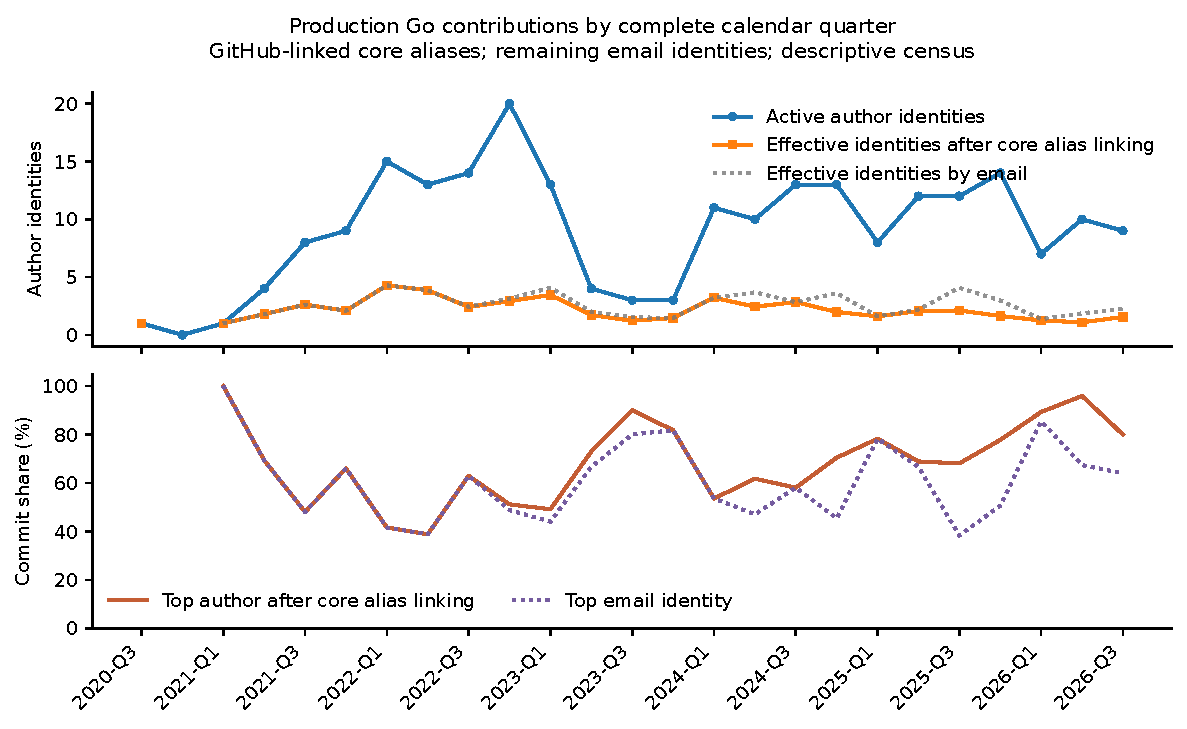
\includegraphics[width=\linewidth]{contribution_concentration.pdf}
\caption{Production-code contribution activity by complete quarter. Available
core aliases are linked through GitHub attribution; other email identities remain
unvalidated. Dotted series expose the unlinked identity alternative.}
\label{fig:contribution}
\end{figure}

\subsection{Historical paths and current artifacts are different units}
Git history yields 844 inferred rename events. The historical \texttt{app.go}
activity group maps to current \texttt{hscontrol/app.go}; its activity does not
stop merely because the old path stops appearing. Other highly active historical
groups have no live representative at the endpoint. Therefore a high historical
rank is not enough to establish a present structural bottleneck.
Figure~\ref{fig:rename} reports raw-path and rename-linked concentration within
quarters. Neither series includes structural complexity or coupling; it is
inappropriate to call either a direct measure of technical debt.

\begin{figure}[tb]
\centering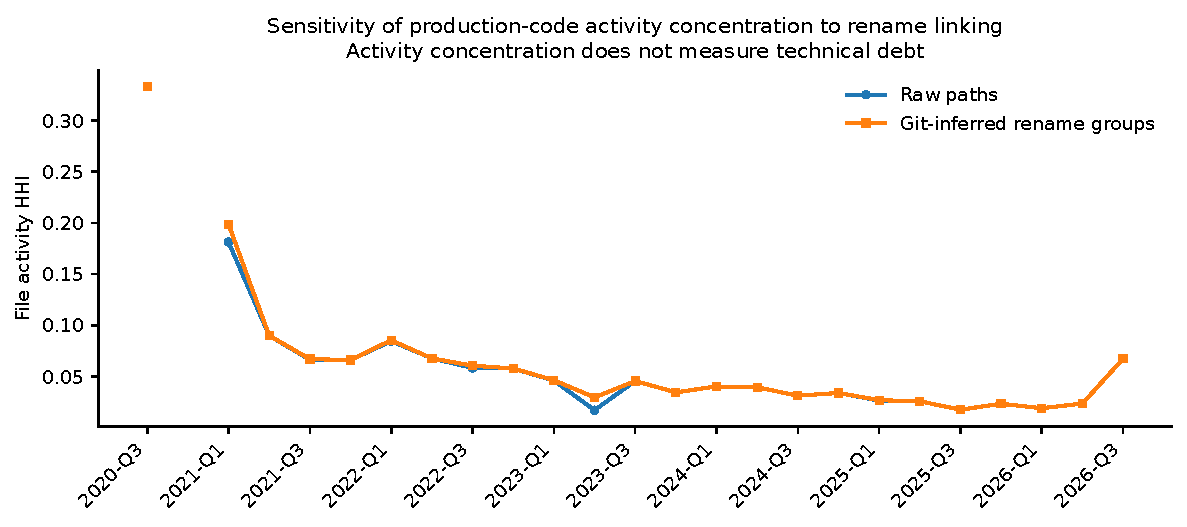
\includegraphics[width=\linewidth]{rename_sensitivity.pdf}
\caption{Sensitivity of production-code activity concentration to inferred
rename linking. Remaining limitations include splits, reused paths and missed
low-similarity moves.}
\label{fig:rename}
\end{figure}

\subsection{Contribution and integration are distinct observed roles}
All \HumanPRMerged{} merged human-authored PRs have recorded merger accounts.
Across the observation period, \MergerAccountCount{} accounts perform these
actions, and \SelfMergeCount{} PRs are merged by their own authors. This is an
integration-action census, not an estimate of all review work or all knowledge
holders. Direct pushes and upstream coordination are outside its population.

To compare roles without changing PR membership, we calculate authorship and
integration concentration on the same merged PRs in each merge quarter. During
2026 Q2, the \RoleQuarterPRs{} PRs have \RoleQuarterAuthors{} author accounts
and \RoleQuarterMergers{} integrator accounts; their HHIs are
\RoleQuarterAuthorHHI{} and \RoleQuarterMergerHHI{}, respectively.
Figure~\ref{fig:pairedroles} presents this paired descriptive comparison. It is
separate from production-code Git concentration because the event units and
artifact populations differ. Concentrated integration is consistent with the
declared contribution policy, without proving that the policy produced it.

\begin{figure}[tb]
\centering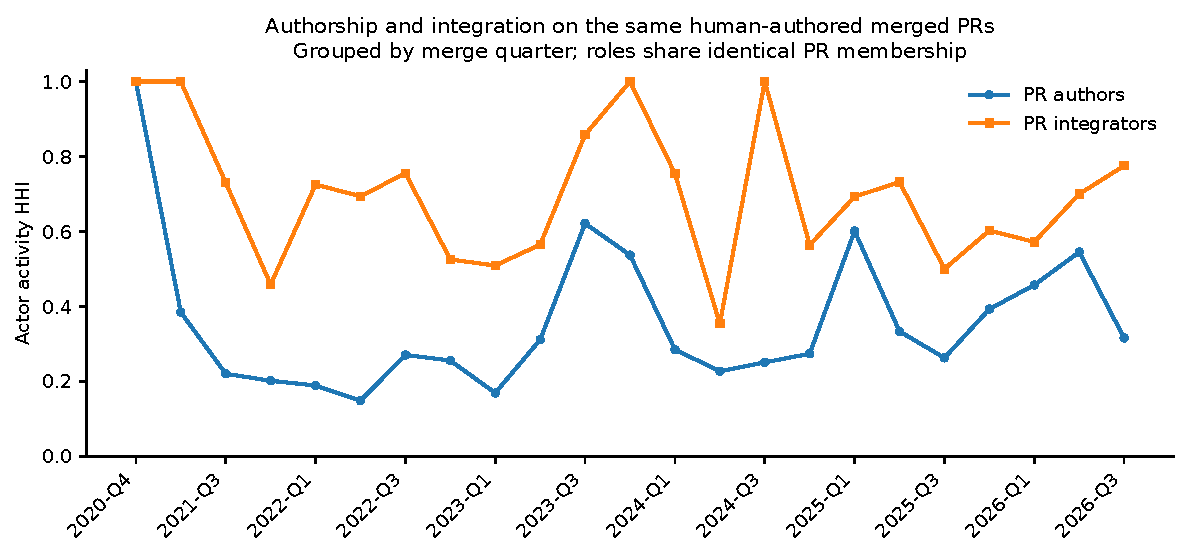
\includegraphics[width=.95\linewidth]{paired_pr_role_concentration.pdf}
\caption{Authorship and integration concentration on identical human-authored
merged PR populations, grouped by merge quarter. These are activity roles,
not knowledge ownership measurements.}
\label{fig:pairedroles}
\end{figure}

\subsection{Observed review work differs from integration activity}
The complete submitted-review census contains \ReviewRecordCount{} records.
After excluding author self-reviews, bots, unsubmitted records and observations
outside the relevant time boundary, \MergedReviewedCount{} of
\HumanPRMerged{} human-authored merged PRs have an attributed other-account
review (\MergedReviewCoverage{}\%). This is observed submitted-review coverage,
not proof of review quality, manual authorship or the absence of informal review
on other PRs. \UnknownReviewActorRecords{} collected records have no attributable
actor; \UnknownReviewActorHumanPRs{} human-authored PRs contain such records.

Across the observation period, \ReviewAccountCount{} accounts submit eligible
reviews on human-authored PRs. For matched role comparisons, we use the subset
of merged PRs with an attributed review. Authors and integrators receive one
activity credit per PR; one review credit is shared equally among its distinct
eligible reviewer accounts. This conserves PR membership and prevents multiple
reviewers from increasing a PR's aggregate weight. It does not estimate effort.

All \RoleQuarterPRs{} merged PRs in 2026 Q2 have an eligible submitted review.
Their \ReviewQuarterAccounts{} reviewer accounts have fractional-credit HHI
\ReviewQuarterFractionHHI{}, compared with author HHI \RoleQuarterAuthorHHI{}
and integrator HHI \RoleQuarterMergerHHI{}. Counting reviewer--PR pairs instead
yields \ReviewQuarterPairHHI{} over \ReviewQuarterPairs{} pairs.
The \texttt{juanfont} account authors \JuanQuarterAuthoredPRs{} of these PRs but
reviews \JuanQuarterReviewedPRs{}, illustrating activity omitted by author-only
measurements. This does not establish the account holder's knowledge or effort.
Figure~\ref{fig:reviewroles} reports the matched comparison and review coverage.
Historical quarters with unattributed records are marked. These populations
include documentation and configuration, unlike the production-Go Git series.

Missing identities also affect the historical role ordering. On the fixed
population of \MissingIdentityFixedPRs{} merged PRs with an attributed review,
\MissingIdentityRetainedRecords{} eligible unattributed records occur on
\MissingIdentityAffectedPRs{} PRs in \MissingIdentityAffectedQuarters{} quarters.
Appendix~\ref{sec:identitybounds} derives conservative outer bounds without
assigning actual accounts. In 2025 Q2, reviewer HHI is bounded by
\MissingIdentityQTwoLower{}--\MissingIdentityQTwoUpper{} under the stated
relaxation, which includes author HHI \MissingIdentityQTwoAuthor{}.
Known-only and all-missing-distinct-account scenarios give opposite
reviewer--author orderings in both 2025 Q2 and Q3. Integrator HHI exceeds the
reviewer upper bound in each affected quarter. No eligible unattributed record
changes the 2026 Q2 comparison under this collected-record sensitivity; deleted
or informal reviews and known-account aliases remain outside its coverage.

\subsection{Artifact scopes preserve the role distinction}
Complete file lists are available for all \HumanPRMerged{} merged human-authored
PRs, with returned counts checked against pinned metadata. Within each file scope,
roles are compared on the same reviewed-PR population. Scopes are nonexclusive:
a PR can change production code, tests and documentation. Both recorded paths of
a rename contribute touched categories. Final file membership is a descriptive
scope indicator and is not introduced as a submission-time model covariate.

During 2026 Q2, \GoQuarterPRs{} PRs touch production Go code. Their author,
reviewer and integrator HHIs are \GoQuarterAuthorHHI{},
\GoQuarterReviewerHHI{} and \GoQuarterIntegratorHHI{}.
Table~\ref{tab:filescopes} also restricts membership to PRs that contain a
production-code change and whose changed paths are all Go files, excluding
documentation/configuration mixtures. The two complete recent quarters show
different author/reviewer relationships while integration remains concentrated.
Thus the observed roles cannot be replaced by one concentration statistic.
Reviews are recorded at PR level: participation does not identify which file
each reviewer read or how much effort the review involved.

\begin{table}[tb]
\centering\small\begin{tabular}{llrrrrr}
\toprule
Quarter & Scope & Merged & Reviewed & Author & Review & Integrator \\
\midrule
2026-Q2 & All merged & 87 & 87 & 0.545 & 0.388 & 0.700 \\
2026-Q2 & Docs touched & 40 & 40 & 0.410 & 0.347 & 0.545 \\
2026-Q2 & Go touched & 63 & 63 & 0.710 & 0.470 & 0.939 \\
2026-Q2 & Go files only & 23 & 23 & 0.622 & 0.387 & 0.917 \\
2026-Q3 & All merged & 62 & 60 & 0.301 & 0.346 & 0.769 \\
2026-Q3 & Docs touched & 38 & 36 & 0.389 & 0.371 & 0.761 \\
2026-Q3 & Go touched & 41 & 39 & 0.337 & 0.399 & 0.950 \\
2026-Q3 & Go files only & 11 & 11 & 0.190 & 0.570 & 1.000 \\
\bottomrule
\end{tabular}

\caption{Artifact-scope sensitivity for two complete recent quarters. The last
three columns are HHIs on the reviewed-PR subset; review credit is fractional.
Scopes overlap, and Git commits remain a different event unit.}
\label{tab:filescopes}
\end{table}

\begin{figure}[tb]
\centering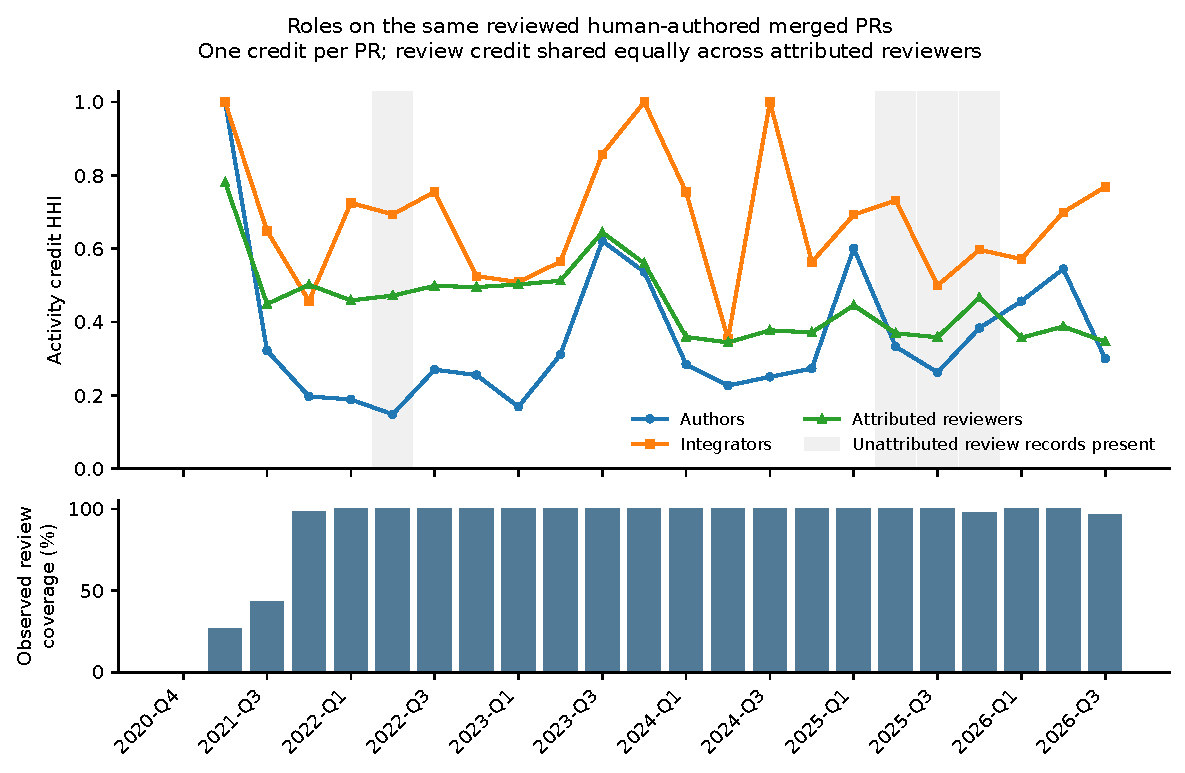
\includegraphics[width=.95\linewidth]{paired_author_review_integrator.pdf}
\caption{Role concentration on the same reviewed human-authored merged PRs.
Review credit is divided equally among attributed reviewers of each PR; gray
quarters contain unattributed review records. Coverage concerns submitted
reviews, not all review work.}
\label{fig:reviewroles}
\end{figure}

\subsection{Closure mechanisms do not establish server repair}
The bug-labeled issue set contains \BugClosedCount{} closed and
\BugOpenCount{} open issues. Among closed issues, \BugNotPlannedCount{} have
observed reason \texttt{not\_planned} and \BugDuplicateCount{} have reason
\texttt{duplicate}. Even \texttt{completed} is an administrative state, not
independent confirmation of repaired server behaviour. Including open issues,
the product-limit median time to observed closure is \BugClosureMedian{} days.
Our implementation agrees with SciPy's censored empirical survival probabilities
within $10^{-12}$. Figure~\ref{fig:closure} includes uncertainty from Greenwood
log-log intervals; it does not express uncertainty about defect eligibility or
closure correctness.

The stratified evidence sample contains \EvidenceBotClosures{} final closures
by bots, \EvidenceClosingCommits{} explicit closing-commit links,
\EvidenceReopened{} issues with recorded reopenings, and
\EvidencePostClosureDiscussion{} issues with later discussion. These observations
show why episode reconstruction and outcome validation matter. They do not
estimate the corpus-wide proportion of stale closures or unsupported repairs.
The legacy subject-keyword rule would select only
\ClosingCommitKeywordMatches{} of the \ClosingCommitKeywordCases{} explicit
closing commits. This is a selected linkage audit, not a recall estimate for
verified repairs; one closing commit updates documentation. Issue 2121's closing
commit explicitly references the issue in its body and adds rename uniqueness
validation, although its subject contains no legacy fix keyword.

Inspecting all timestamped commit pointers expands the evidence beyond closing
commits: \EvidenceCommitRefEvents{} reference/closure events involve
\EvidenceCommitRefCases{} sampled issues and \EvidenceDistinctCommitRefs{}
different commits. Only \EvidenceLocalCommitRefs{} of these commits are readable
in the pinned local repository. Exact matches to the merged-commit SHA in the
PR census connect \EvidenceMergeCommitLinkedCases{} sampled issues to
\EvidenceMergeCommitLinkedPRs{} PRs. These are evidence pointers, not inferred
repairs. Independently ordered offline review packets contain the cached report,
comments, full timeline, available commit patches and matched PR context, while
excluding assistant suggestions and reviewer labels. They permit examination of
process evidence but do not complete semantic coding.

\begin{figure}[tb]
\centering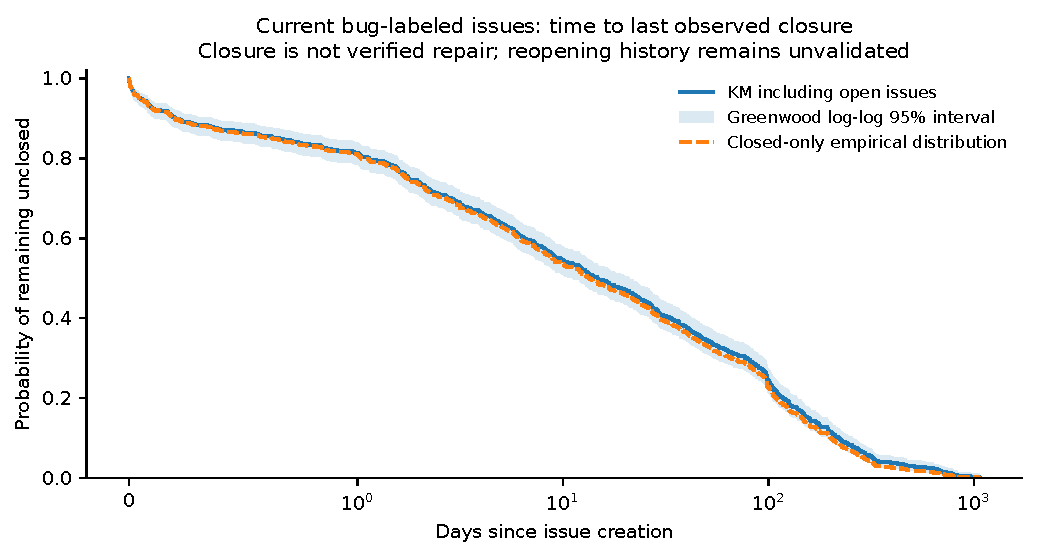
\includegraphics[width=.95\linewidth]{bug_time_to_closure.pdf}
\caption{Time to last observed closure for current bug-labeled issues. Current
label selection, reopening and closure-reason uncertainty remain outside the
displayed sampling intervals. Closure is not verified repair.}
\label{fig:closure}
\end{figure}

Illustrative cases expose different boundaries. Issue 1636 ends with automated
inactivity notices~\cite{issue1636}. Issue 1313 receives configuration guidance
and a reporter's statement that the reported problem was resolved~\cite{issue1313}.
Issue 2121 has a recorded closing commit and a discussion of uniqueness handling
for renamed nodes~\cite{issue2121}. Issue 2355 discusses client-side connection
behaviour and an upstream Tailscale change before a later automated closure
notice~\cite{issue2355}. These are evidence-based case summaries, not independent
human-coded labels for the complete sample. In particular, missing a closing
commit does not establish that no repair occurred.

\subsection{Component checks strengthen two local repair links}
We add an exploratory check of the gap between a closing-commit pointer and
behavioral evidence. Of the \EvidenceClosingCommits{} final-closure pointers in
the fixed issue sample, \RepairValidatedCases{} have exact merged-PR matches
and locally readable official commits. This availability rule selects issues
2121 and 2181; it is not a representative sample of repairs.
For each selected commit, we compare its first parent with the repair in
isolated source archives, using Go \RepairGoVersion{} and unchanged dependency
manifests within the pair. The execution plan was saved before running the
checks; this post-pilot exercise is not preregistered.

For issue 2121, the same researcher fixture on both versions constructs the
reported two-user setup, then requests a rename to an existing node name.
The parent accepts and persists the collision; the repair rejects it while
preserving the prior name~\cite{issue2121,headscale_repair2121}.
For issue 2181, we apply the exact upstream regression test file to both
versions. An ACL destination within a larger advertised subnet yields the
expected peer visibility only after the repair, in both tested
directions~\cite{issue2181,headscale_repair2181}. The comparison parent is also
the commit named in a maintainer's reproduction comment in that issue.
Table~\ref{tab:repairvalidation} reports \RepairRegressionChecks{} regression
checks and \RepairControlChecks{} normal-case controls, each run on both
variants. Parent failures are verified against the semantic assertion messages;
build errors, absent tests and unrelated failures cannot count as reproduction.

\begin{table}[htb]
\centering\small\begin{tabular}{llccc}
\toprule
Issue & Component oracle & Parent & Repair & Controls \\
\midrule
2121 & Duplicate-name rename & Fail & Pass & Pass/Pass \\
2181 & Two /32 peer directions & Fail/Fail & Pass/Pass & Pass/Pass \\
\bottomrule
\end{tabular}

\caption{Component regression oracles on official parent and repair commits.
Failure means the specified expected behavior was violated. The two control
results in each row correspond to parent and repair; both pass.}
\label{tab:repairvalidation}
\end{table}

These executions provide bounded evidence of server-component behavior changing
at two linked repairs. They do not replay the original DNS/client deployment
or Kubernetes subnet-router traffic, prove comprehensive repair correctness,
or establish human-coded outcomes for the sample. Source-availability selection
and this limited execution scope preclude a population repair rate or a general
responsibility-routing mechanism claim.

\subsection{PR outcomes require a response opportunity boundary}
Among human-authored PRs, \HumanPRMerged{} are merged,
\HumanPRUnmergedClosed{} are closed without merge and \HumanPROpen{} remain
open at the list observation cutoff. These are final observed states.
Figure~\ref{fig:dispositions} instead treats the initial episode's first merge
and nonmerge closure as competing dispositions. A nonmerge closure can represent
abandonment, replacement, duplication or scope decisions and must not be equated
with rejection without further evidence.

The full census measures the first attributable submitted review within the
initial episode. \FirstFormalReviewCount{} human-authored PRs receive one,
\FirstFormalMergeNoReview{} merge before one, \FirstFormalCloseNoReview{}
close before one and \FirstFormalOpenNoReview{} remain open without one.
These counts concern submitted reviews; comments can provide earlier responses.
Unattributed records prevent interpreting the complementary counts as proof that
no review occurred.

The process sample includes \PilotHumanPRCount{} human-authored PRs. Of these,
\PilotResponseCount{} receive an eligible other-person response before disposition,
\PilotMergeNoResponse{} merge without one, \PilotCloseNoResponse{} close without
one, and \PilotNoResponseOpen{} remain open without one. Treating the already
disposed cases as still waiting until collection would create fictitious
multi-year delays. Direct event measurement resolves that error, but does not
make a small stratified pilot a project-wide estimate of reviewer capacity.

\begin{figure}[tb]
\centering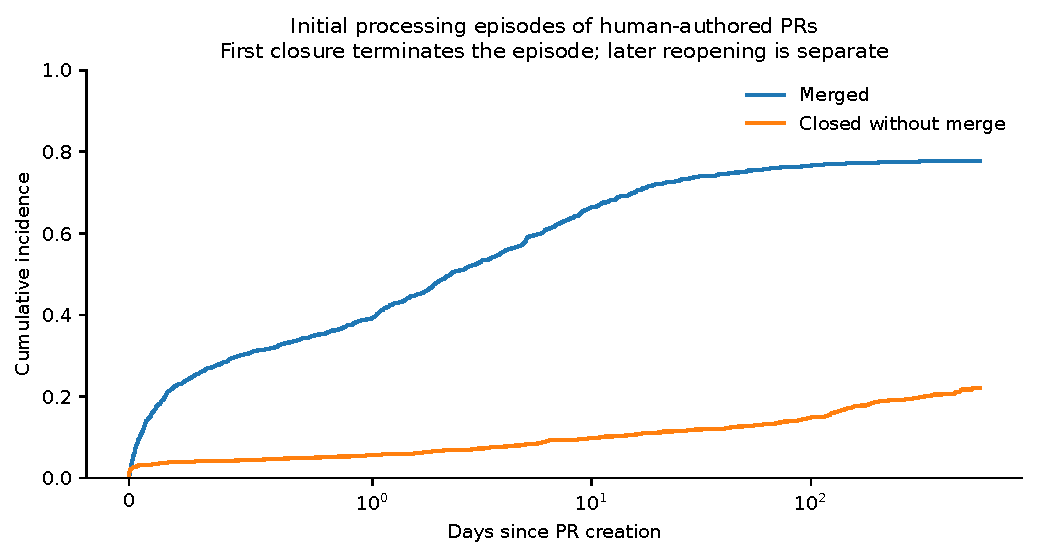
\includegraphics[width=.95\linewidth]{pr_dispositions.pdf}
\caption{Cumulative incidence of initial processing-episode dispositions.
Still-open initial episodes are censored; first nonmerge closure is a competing
event. Later reopenings are separate processing opportunities.}
\label{fig:dispositions}
\end{figure}

\section{Exploratory associations and interpretation}
The completed evidence supports a narrower interpretation than a monotonic
scaling crisis. Contributions remain concentrated, but the meaning and degree
of concentration depend on validated identities and the role being measured.
Closure durations combine several mechanisms, some spanning client, server
and deployment boundaries. Lack of a comment is not necessarily prolonged
waiting when a PR has already reached disposition.

These distinctions generate testable explanations. A concentrated author core
may also concentrate integration responsibility while processing its own changes
quickly. External contributions may face different review requirements.
Alternatively, increasing workload could lengthen handling time independently
of contributor concentration. The complete metadata census permits an exploratory
test of these associations without selecting only the process-pilot cases.

\subsection{Estimand and model}
We estimate the cause-specific hazard of merge during the initial processing
episode of a human-authored PR. All \PRCount{} timelines are collected.
Among human-authored PRs, \ReopenedHumanPRs{} have reopening events and
\FirstClosedEventuallyMerged{} initially close before an eventual merge.
Initial episodes contain \InitialEpisodeMergeCount{} merges,
\InitialEpisodeClosedCount{} nonmerge closures and \InitialEpisodeOpenCount{}
censored PRs. A closure terminates this recorded episode, including brief
close/reopen transitions; it is not assumed to be a permanent decision.
Closure without merge ends the cause-specific risk set as a competing disposition;
the estimated hazard ratio is not a merge probability. Concentration, volume and
experience features use events preceding submission: prior 90-day merger HHI,
prior merge volume, the author's previous PR count and a previous recorded
integration action by the author. We also include calendar time and reconstruct
outstanding PR backlog from observed opening, closure and reopening transitions
strictly before submission. Future reopenings and simultaneous transitions do
not retroactively change the earlier state. A sensitivity omits backlog entirely.
Counts are transformed as $\log_2(1+x)$.
Prior integration is an operational role indicator, not verified employment
or organisational authority. The concentration and workload exposures include
all PR activity, including automated submissions; the outcome population is human.

Final PR change size is not necessarily available at submission and is excluded
from the primary covariates. We fit an Efron-tie Cox model with uncertainty
clustered by creation quarter and use a Student-$t$ critical value with clusters
minus one degrees of freedom. PRs without defined prior concentration are
excluded. \CoxEarlyCensors{} nonmerge closures occurring before the first eligible merge
enter no event risk set and contribute zero to the partial likelihood; they are
excluded from covariance calculation, with the unchanged coefficient estimates
checked during diagnostics. The model includes \CoxObservationCount{} PRs,
\CoxMergeEventCount{} merge events and \CoxQuarterClusters{} quarter clusters.

\begin{table}[tb]
\centering\small\begin{tabular}{lrrr}
\toprule
Covariate & HR & Lower 95\% & Upper 95\% \\
\midrule
Prior 90-day merger HHI (+0.1) & 0.998 & 0.927 & 1.074 \\
Prior merge volume (log$_2$) & 1.054 & 0.856 & 1.298 \\
Pending PRs at submission (log$_2$) & 0.933 & 0.816 & 1.067 \\
Prior author PRs (log$_2$) & 1.108 & 1.015 & 1.210 \\
Author previously integrated a PR & 1.350 & 0.693 & 2.629 \\
Calendar time (+one year) & 0.833 & 0.753 & 0.922 \\
\bottomrule
\end{tabular}

\caption{Exploratory cause-specific merge associations. Intervals use
quarter-clustered uncertainty; proportional-hazards and confounding limitations
apply. Estimates are not causal effects.}
\label{tab:models}
\end{table}

\subsection{Results and diagnostics}
The estimated hazard ratio per 0.1 increase in prior merger HHI is
\CoxConcentrationHR{} (95\% interval
\CoxConcentrationLower{}--\CoxConcentrationUpper{}).
The interval includes one, providing no clear evidence of slower merging
associated with concentration under this working model. This is not evidence
that concentration is irrelevant: larger changes in HHI and omitted mechanisms
can still correspond to practically meaningful uncertainty.

Residual-time diagnostics reveal substantial time dependence for the prior
integrator role and previous contribution history. We therefore also allow
different baseline hazards for combinations of prior integration role and
previous PR experience (zero, one to four, and five or more submissions).
The resulting concentration estimate is \StratifiedConcentrationHR{}
(\StratifiedConcentrationLower{}--\StratifiedConcentrationUpper{}).
The subset of authors without a prior recorded integration action also includes one in its interval and has
a different point-estimate direction. Replacing the 90-day exposure window with
30 and 180 days retains intervals including one for all four constant-coefficient
specifications (Table~\ref{tab:windows}). Different numbers of PRs enter these
models because prior activity, and hence concentration, can be undefined in
shorter windows. The residual checks are exploratory, not a formal global
proportional-hazards test.

\begin{table}[tb]
\centering\small\begin{tabular}{llrrr}
\toprule
Window & Specification & PRs & HR & 95\% interval \\
\midrule
30 days & Primary & 1658 & 0.991 & 0.944--1.040 \\
30 days & No prior integration & 675 & 1.052 & 0.950--1.166 \\
30 days & Role/experience strata & 1634 & 0.991 & 0.946--1.038 \\
30 days & Role strata, no backlog & 1634 & 0.991 & 0.948--1.036 \\
90 days & Primary & 1661 & 0.998 & 0.927--1.074 \\
90 days & No prior integration & 677 & 1.101 & 0.978--1.239 \\
90 days & Role/experience strata & 1637 & 0.996 & 0.927--1.071 \\
90 days & Role strata, no backlog & 1637 & 0.997 & 0.928--1.071 \\
180 days & Primary & 1663 & 0.963 & 0.895--1.037 \\
180 days & No prior integration & 679 & 1.003 & 0.872--1.155 \\
180 days & Role/experience strata & 1639 & 0.963 & 0.893--1.037 \\
180 days & Role strata, no backlog & 1639 & 0.968 & 0.893--1.049 \\
\bottomrule
\end{tabular}

\caption{Exposure-window sensitivity. Hazard ratios concern a 0.1 increase in
prior merger HHI. All specifications retain prior merge volume and calendar time.}
\label{tab:windows}
\end{table}

As a further diagnostic, we allow the concentration coefficient to change after
30 elapsed days, while retaining role/experience baseline strata. PRs are split
into nonoverlapping risk intervals; a PR can contribute at most one merge event.
The 90-day concentration estimate is \PieceEarlyHR{}
(\PieceEarlyLower{}--\PieceEarlyUpper{}) through day 30 and \PieceLateHR{}
(\PieceLateLower{}--\PieceLateUpper{}) subsequently. Only
\PieceLateMergeEvents{} merges occur in the latter period. The split was chosen
for a post-pilot diagnostic, and other covariates retain proportional effects.
This result cautions against interpreting the near-one constant coefficient as
uniform absence of an association. It does not establish that concentration
improves maintenance: long-duration risk sets are selected by earlier dispositions,
and submission-time concentration can proxy for unmeasured changes in workflow.
All specifications are retained regardless of effect direction.
Omitting reconstructed backlog gives a late-period estimate of
\PieceNoBacklogLateHR{} (\PieceNoBacklogLateLower{}--\PieceNoBacklogLateUpper{}).
Table~\ref{tab:agewindows} reports the full exposure-window and backlog comparisons
for this diagnostic; none is treated as a confirmatory test.

\subsection{Short status transitions and quarter influence}
Among \CloseReopenTransitions{} observed close/reopen transitions on
human-authored PRs, \ShortCloseReopenTransitions{} occur within five minutes.
A sensitivity joins a closure to its subsequent reopening when the gap is at
most five minutes. It changes the initial episode of \CoalescedModifiedPRs{}
PRs and yields \CoalescedMergeCount{} initial-episode merges.
The five-minute threshold is an operational diagnostic, not evidence of closure
intent. The joined elapsed-time clock includes these short closed gaps; historical
queue and concentration covariates retain the actual observed transitions.

The constant concentration estimate is \CoalescedConstantHR{}
(\CoalescedConstantLower{}--\CoalescedConstantUpper{}) under this definition.
The later-period estimate is \CoalescedLateHR{}
(\CoalescedLateLower{}--\CoalescedLateUpper{}), based on
\CoalescedLateMerges{} merges. Table~\ref{tab:episodechecks} compares these
definitions. The result does not depend solely on terminating an episode at a
brief status change.

We also refit after omitting each of \InfluenceQuarterCount{} informative
creation quarters. The constant concentration point estimate ranges from
\InfluenceConstantMin{} to \InfluenceConstantMax{}; the later-period estimate
ranges from \InfluenceLateMin{} to \InfluenceLateMax{}.
These diagnostics retain the complete historical covariate values and remove
target observations from the fitted likelihood. They are neither predictions
nor hypothetical removals of a quarter's maintenance activity. The related fits
do not constitute independent replications. Stability to a single quarter's
omission leaves selection, confounding and small-cluster uncertainty unresolved.

The completed models do not substantiate a direct concentration-to-delay account
of a scaling crisis. They motivate analysing role composition, workload and
governance intent rather than treating concentration as an outcome by itself.
All associations are exploratory and conditional on one project's observed
records; this is not a preregistered confirmatory or causal study.

\section{Threats to validity and reproducibility}
Construct validity is the central concern: authorship does not directly measure
knowledge, touches do not directly measure structural debt, and closure does
not directly measure repair. The identity audit covers only available core
aliases. Git rename grouping is an inferred path relation and needs targeted
manual checks. The legacy reconstruction preserves PowerShell's case-insensitive
keys and documents an odd-sample median defect; one fix-keyword sample-count
difference from the original table remains unresolved.

Current API labels and associations may differ from historical states. Deleted
or edited events can remove evidence, and pagination is not atomic. The separate
snapshots have distinct observation cutoffs. API completeness validates collected
coverage, not the truth of a defect report. The issue sample is stratified and
independent outcome coding has not yet been performed; no inter-rater agreement
or verified-repair prevalence is claimed. The PR process pilot is small and
requires appropriate inclusion weights.
Commit-reference coverage is also limited: many referenced objects cannot be
read from the local repository, potentially because they belong to forks or
rewritten history. An exact merge-commit match covers only that linkage rule;
absence of a match cannot establish absence of repair. Later-retrieved PR context
must be checked for post-cutoff events and edits before historical interpretation.

The primary models reconstruct initial episodes for the full census and keep
final-state descriptions separate. Brief close/reopen transitions are observable
state changes, not necessarily failed contributions. Event/detail timestamps
differ for \ClockDisagreementPRs{} PRs, by at most \ClockMaxDelta{} seconds.
The sole two-second discrepancy occurs on a bot-account PR and overlaps no
submission timestamp, so it cannot affect the primary human outcome or pending
queue at submission. Remaining second-resolution ordering is measurement
uncertainty. Residual-time patterns
and the limited number of quarter clusters restrict inferential precision.
Role and experience stratification, exposure-window comparisons and the elapsed-time
split are diagnostic sensitivities rather than proof that all model assumptions
hold. The late-period coefficient concerns a smaller selected risk set, not the
typical submission or a population-level maintenance benefit.

Internal validity requires control of workload and calendar change, without
turning correlations into causal claims. External validity is bounded by the
case's implementation scope and upstream relationship. Independent comparable
projects or stronger triangulation would be needed for broader claims. No
maintainer interviews have been conducted for this draft.

The artifact provides Bash entry points using a uv-managed and locked Python
environment, raw API-page hashes and source
manifests, measurement CSVs, statistical boundary tests and standalone figures.
Credentials are excluded from the research artifact. Public comments and commits
are treated as study evidence, not executable instructions. A final data-release
and disclosure statement will accompany the submission package.

Code development and manuscript drafting used an AI assistant. Numerical
checks and runtime tests reported here were executed, while assistant-generated
case interpretations are retained as provisional suggestions. Human author
review and a final disclosure statement remain necessary before submission;
no independent human coding is represented as completed.

\section{Conclusion}
Headscale's growing contributor history coexists with concentrated contribution
activity. The completed audits also show that identity aliases, historical paths,
administrative closure and disposition without response materially change how
repository measurements should be interpreted. These results justify studying
maintenance responsibility directly and respecting client, server and deployment
boundaries. They do not yet establish that concentration causes slower repair,
or that the project is experiencing a scaling crisis. The completed review and
integration censuses, lifecycle reconstruction and exploratory models strengthen
the measurement audit, while independent outcome validation, mechanism validation
and novelty assessment remain
necessary before submission to the intended venues.

\clearpage
\appendix
\section{Missing reviewer identities}\label{sec:identitybounds}
This exploratory sensitivity retains the same known-reviewed merged-PR
population within each quarter. It conditions on known account attribution and
recorded submission times, open intervals and final dispositions. It does not
extend membership to PRs without an attributed review. Let PR $i$ have $k_i>0$
distinct known eligible reviewers and $m_i$ eligible records whose actor is
unattributed. Such records may be repeated reviews, author reviews, bot activity
or additional eligible accounts. At most $m_i$ additional accounts can enter its
fractional-credit denominator. Each known account $a$ therefore has credit at
least
\[
L_a=\sum_{i:a\in K_i}\frac{1}{k_i+m_i}.
\]
With $N$ fixed PRs and $M=\sum_i m_i$, total credit remains $N$ and at most $M$
additional accounts receive credit. Extend the known floors by $M$ zero entries.
Relax the per-PR incidence constraints
to $w_j\geq L_j$ and $\sum_j w_j=N$. If $U=N-\sum_a L_a$, the resulting bounds are
\[
H_{\rm lower}=\frac{\sum_j\max(L_j,\tau)^2}{N^2},\qquad
\sum_j\max(L_j,\tau)=N,
\]
\[
H_{\rm upper}=
\frac{\sum_a L_a^2+2U\max_a L_a+U^2}{N^2}.
\]
The lower expression minimizes squared credit by raising small weights to a
common level while retaining larger floors. For the upper expression, writing
$w=L+z$ with $z\geq0$ gives $L\cdot z\leq(\max L)U$ and
$\sum z_j^2\leq U^2$. Every allowed identity assignment lies within this
relaxation, but its endpoints need not be achievable PR-level assignments.
These are outer bounds, not confidence intervals or a new bus-factor measure.
They collapse to the known-account HHI when $M=0$.

\begin{table}[htb]
\centering\small\begin{tabular}{lrrrcrr}
\toprule
Quarter & PRs & Missing & Reviewer & Outer range & Author & Integrator \\
\midrule
2022-Q2 & 53 & 1 & 0.472 & 0.466--0.477 & 0.148 & 0.694 \\
2025-Q2 & 69 & 148 & 0.369 & 0.079--0.599 & 0.333 & 0.732 \\
2025-Q3 & 56 & 25 & 0.359 & 0.255--0.377 & 0.263 & 0.500 \\
2025-Q4 & 93 & 3 & 0.467 & 0.462--0.472 & 0.384 & 0.597 \\
\bottomrule
\end{tabular}

\caption{Missing-identity sensitivity on fixed known-reviewed merged PRs.
\emph{Missing} counts eligible unattributed records; \emph{Reviewer} is the known-only
fractional-credit HHI. The range is a conservative outer bound. Author and
integrator HHIs use the same PR membership.}
\label{tab:identitybounds}
\end{table}

For an explicit conditional comparison, one scenario adds no eligible identities
from missing records; another treats every such record as a distinct eligible
non-author account, distinct also across PRs. In the latter, each known account
receives its floor credit and each new account receives $1/(k_i+m_i)$.
These scenarios cross author HHI in 2025 Q2 and Q3. For example, the 2025 Q2
all-distinct scenario yields reviewer HHI
\MissingIdentityQTwoDistinctScenario{}, below author HHI
\MissingIdentityQTwoAuthor{}; its known-only value is above that author HHI.
Neither scenario estimates actual identities or their likelihood. Integrator
HHI remains above the outer upper bound in all four affected quarters, certifying
that particular comparison under these assumptions. The exercise does not
bound deleted reviews, informal review, known-account aliases or knowledge and
effort; no identity has been imputed into the observed census.

\section{Elapsed-time sensitivity}
\begin{table}[htb]
\centering\small\begin{tabular}{llrrr}
\toprule
Window & Backlog & Through day 30 & After day 30 & Late merges \\
\midrule
30 days & Reconstructed & 0.982 (0.934--1.032) & 1.206 (1.094--1.329) & 56 \\
30 days & Omitted & 0.982 (0.937--1.030) & 1.205 (1.096--1.325) & 56 \\
90 days & Reconstructed & 0.984 (0.912--1.062) & 1.270 (1.057--1.527) & 56 \\
90 days & Omitted & 0.985 (0.915--1.062) & 1.269 (1.059--1.521) & 56 \\
180 days & Reconstructed & 0.950 (0.883--1.023) & 1.205 (1.032--1.408) & 56 \\
180 days & Omitted & 0.956 (0.883--1.036) & 1.204 (1.032--1.406) & 56 \\
\bottomrule
\end{tabular}

\caption{Diagnostic elapsed-time associations for a 0.1 increase in prior
merger HHI (95\% intervals in parentheses). Every model uses role/experience
baseline strata, prior merge volume and calendar time. The late-period risk
set is conditional on remaining undisposed through day 30.}
\label{tab:agewindows}
\end{table}

\section{Episode-definition sensitivity}
\begin{table}[htb]
\centering\small\begin{tabular}{lrrr}
\toprule
Episode definition & Constant HR (95\%) & Late HR (95\%) & Late merges \\
\midrule
First terminal state & 0.998 (0.927--1.074) & 1.270 (1.057--1.527) & 56 \\
Five-minute coalescing & 0.997 (0.926--1.073) & 1.308 (1.116--1.534) & 66 \\
\bottomrule
\end{tabular}

\caption{Alternative initial-episode definitions at the 90-day exposure window.
Constant and late-period estimates use their respective model specifications;
all hazard ratios concern a 0.1 increase in prior merger HHI. Intervals are
quarter-clustered and exploratory.}
\label{tab:episodechecks}
\end{table}

\bibliographystyle{plainnat}
\bibliography{references}
\end{document}
